\documentclass[]{article}
\usepackage{lmodern}
\usepackage{amssymb,amsmath}
\usepackage{ifxetex,ifluatex}
\usepackage{fixltx2e} % provides \textsubscript
\ifnum 0\ifxetex 1\fi\ifluatex 1\fi=0 % if pdftex
  \usepackage[T1]{fontenc}
  \usepackage[utf8]{inputenc}
\else % if luatex or xelatex
  \ifxetex
    \usepackage{mathspec}
  \else
    \usepackage{fontspec}
  \fi
  \defaultfontfeatures{Ligatures=TeX,Scale=MatchLowercase}
\fi
% use upquote if available, for straight quotes in verbatim environments
\IfFileExists{upquote.sty}{\usepackage{upquote}}{}
% use microtype if available
\IfFileExists{microtype.sty}{%
\usepackage{microtype}
\UseMicrotypeSet[protrusion]{basicmath} % disable protrusion for tt fonts
}{}
\usepackage[margin=1in]{geometry}
\usepackage{hyperref}
\hypersetup{unicode=true,
            pdftitle={Scarid grazing behavior - manuscript draft},
            pdfauthor={Molly Wilson},
            pdfborder={0 0 0},
            breaklinks=true}
\urlstyle{same}  % don't use monospace font for urls
\usepackage{color}
\usepackage{fancyvrb}
\newcommand{\VerbBar}{|}
\newcommand{\VERB}{\Verb[commandchars=\\\{\}]}
\DefineVerbatimEnvironment{Highlighting}{Verbatim}{commandchars=\\\{\}}
% Add ',fontsize=\small' for more characters per line
\usepackage{framed}
\definecolor{shadecolor}{RGB}{248,248,248}
\newenvironment{Shaded}{\begin{snugshade}}{\end{snugshade}}
\newcommand{\KeywordTok}[1]{\textcolor[rgb]{0.13,0.29,0.53}{\textbf{#1}}}
\newcommand{\DataTypeTok}[1]{\textcolor[rgb]{0.13,0.29,0.53}{#1}}
\newcommand{\DecValTok}[1]{\textcolor[rgb]{0.00,0.00,0.81}{#1}}
\newcommand{\BaseNTok}[1]{\textcolor[rgb]{0.00,0.00,0.81}{#1}}
\newcommand{\FloatTok}[1]{\textcolor[rgb]{0.00,0.00,0.81}{#1}}
\newcommand{\ConstantTok}[1]{\textcolor[rgb]{0.00,0.00,0.00}{#1}}
\newcommand{\CharTok}[1]{\textcolor[rgb]{0.31,0.60,0.02}{#1}}
\newcommand{\SpecialCharTok}[1]{\textcolor[rgb]{0.00,0.00,0.00}{#1}}
\newcommand{\StringTok}[1]{\textcolor[rgb]{0.31,0.60,0.02}{#1}}
\newcommand{\VerbatimStringTok}[1]{\textcolor[rgb]{0.31,0.60,0.02}{#1}}
\newcommand{\SpecialStringTok}[1]{\textcolor[rgb]{0.31,0.60,0.02}{#1}}
\newcommand{\ImportTok}[1]{#1}
\newcommand{\CommentTok}[1]{\textcolor[rgb]{0.56,0.35,0.01}{\textit{#1}}}
\newcommand{\DocumentationTok}[1]{\textcolor[rgb]{0.56,0.35,0.01}{\textbf{\textit{#1}}}}
\newcommand{\AnnotationTok}[1]{\textcolor[rgb]{0.56,0.35,0.01}{\textbf{\textit{#1}}}}
\newcommand{\CommentVarTok}[1]{\textcolor[rgb]{0.56,0.35,0.01}{\textbf{\textit{#1}}}}
\newcommand{\OtherTok}[1]{\textcolor[rgb]{0.56,0.35,0.01}{#1}}
\newcommand{\FunctionTok}[1]{\textcolor[rgb]{0.00,0.00,0.00}{#1}}
\newcommand{\VariableTok}[1]{\textcolor[rgb]{0.00,0.00,0.00}{#1}}
\newcommand{\ControlFlowTok}[1]{\textcolor[rgb]{0.13,0.29,0.53}{\textbf{#1}}}
\newcommand{\OperatorTok}[1]{\textcolor[rgb]{0.81,0.36,0.00}{\textbf{#1}}}
\newcommand{\BuiltInTok}[1]{#1}
\newcommand{\ExtensionTok}[1]{#1}
\newcommand{\PreprocessorTok}[1]{\textcolor[rgb]{0.56,0.35,0.01}{\textit{#1}}}
\newcommand{\AttributeTok}[1]{\textcolor[rgb]{0.77,0.63,0.00}{#1}}
\newcommand{\RegionMarkerTok}[1]{#1}
\newcommand{\InformationTok}[1]{\textcolor[rgb]{0.56,0.35,0.01}{\textbf{\textit{#1}}}}
\newcommand{\WarningTok}[1]{\textcolor[rgb]{0.56,0.35,0.01}{\textbf{\textit{#1}}}}
\newcommand{\AlertTok}[1]{\textcolor[rgb]{0.94,0.16,0.16}{#1}}
\newcommand{\ErrorTok}[1]{\textcolor[rgb]{0.64,0.00,0.00}{\textbf{#1}}}
\newcommand{\NormalTok}[1]{#1}
\usepackage{graphicx,grffile}
\makeatletter
\def\maxwidth{\ifdim\Gin@nat@width>\linewidth\linewidth\else\Gin@nat@width\fi}
\def\maxheight{\ifdim\Gin@nat@height>\textheight\textheight\else\Gin@nat@height\fi}
\makeatother
% Scale images if necessary, so that they will not overflow the page
% margins by default, and it is still possible to overwrite the defaults
% using explicit options in \includegraphics[width, height, ...]{}
\setkeys{Gin}{width=\maxwidth,height=\maxheight,keepaspectratio}
\IfFileExists{parskip.sty}{%
\usepackage{parskip}
}{% else
\setlength{\parindent}{0pt}
\setlength{\parskip}{6pt plus 2pt minus 1pt}
}
\setlength{\emergencystretch}{3em}  % prevent overfull lines
\providecommand{\tightlist}{%
  \setlength{\itemsep}{0pt}\setlength{\parskip}{0pt}}
\setcounter{secnumdepth}{0}
% Redefines (sub)paragraphs to behave more like sections
\ifx\paragraph\undefined\else
\let\oldparagraph\paragraph
\renewcommand{\paragraph}[1]{\oldparagraph{#1}\mbox{}}
\fi
\ifx\subparagraph\undefined\else
\let\oldsubparagraph\subparagraph
\renewcommand{\subparagraph}[1]{\oldsubparagraph{#1}\mbox{}}
\fi

%%% Use protect on footnotes to avoid problems with footnotes in titles
\let\rmarkdownfootnote\footnote%
\def\footnote{\protect\rmarkdownfootnote}

%%% Change title format to be more compact
\usepackage{titling}

% Create subtitle command for use in maketitle
\newcommand{\subtitle}[1]{
  \posttitle{
    \begin{center}\large#1\end{center}
    }
}

\setlength{\droptitle}{-2em}

  \title{Scarid grazing behavior - manuscript draft}
    \pretitle{\vspace{\droptitle}\centering\huge}
  \posttitle{\par}
    \author{Molly Wilson}
    \preauthor{\centering\large\emph}
  \postauthor{\par}
      \predate{\centering\large\emph}
  \postdate{\par}
    \date{Nov. 2018}


\begin{document}
\maketitle

{
\setcounter{tocdepth}{2}
\tableofcontents
}
\section{Intro + motivation}\label{intro-motivation}

\begin{itemize}
\tightlist
\item
  Grazing by herbivorous fish is an established driver of coral reef
  health/benthic dynamics
\item
  As reefs become increasingly degraded/threatened, there is growing
  interest in understanding how much herbivory is needed to sustain
  coral reef health (e.g.~herbivore threshold papers - Karr et al. 2015,
  McClanahan et al. 2011)
\item
  However, not all herbivores are the same in terms of their grazing
  impact\ldots{}

  \begin{itemize}
  \tightlist
  \item
    Recent developments in functional classifications, difference across
    species in terms of feeding selectivity, morphology, etc. (e.g.~Adam
    et al. 2018)
  \end{itemize}
\item
  In addition to these inter-species differences in functional role,
  differences in herbivore behavior also affect grazing impact and may
  drive variation in herbivore function among individuals or across reef
  systems
\item
  Previous work has shown that herbivore behavior is sensitive
  to\ldots{}

  \begin{itemize}
  \tightlist
  \item
    Predator presence (and reef structure) (Catano, Madin)
  \item
    Presence of other herbivores (Gil)
  \item
    Resource availability + distribution (Carlson, Tootell, Mumby, etc.)
  \end{itemize}
\item
  In understanding and predicting herbivore impact on reefs, current
  assumption is that grazing behaviors are constant within species (same
  species-level length\textasciitilde{}feeding rate relationships)
\item
  But there is very limited data on how herbivore feeding behaviors
  might vary across reef systems and whether we can accurately assume
  constant species roles at regional scales
\item
  Here we document variability in multiple components (\emph{if I
  include foraging intensity as well as feeding rate\ldots{}}) of scarid
  feeding behavior across reef sites in three Caribbean islands and
  discuss potential underlying mechanisms, ecological consequences, and
  management implications
\item
  We demonstrate a need for further experimental and modelling work to
  unpack these drivers and understand their ecological consequences
\item
  We urge for the incorporation of behavioral effects in coral reef
  herbivore management and caution against assuming constant species
  function across reef systems
\end{itemize}

\section{Methods}\label{methods}

\subsection{Data collection}\label{data-collection}

\begin{itemize}
\tightlist
\item
  Sites (13 sites, 3 islands {[}map{]}), timeline of data collection
\item
  Fish and benthic community surveys
\item
  Observational behavioral data:

  \begin{itemize}
  \tightlist
  \item
    Species: \emph{Sparisoma viride} and \emph{Scarus vetula}, initial
    and terminal phase greater than 15cm
  \item
    2 minute follows, calibration period, outside of previously
    established FID
  \item
    Recording time budgets as well as bite rates during grazing forays
    (define)
  \item
    Discarded data of incomplete follows or where fish were visably
    disturbed/fled
  \item
    Timing of data collection distributed throughout day, 2 dives per
    site
  \item
    Define behavioral variables ({[}table{]})
  \end{itemize}
\end{itemize}

\subsection{Analysis}\label{analysis}

\begin{itemize}
\tightlist
\item
  Fish biomass using lenth-weight conversions (appendix)
\item
  (stats for inter-island differences?)
\item
  PCA of site-level benthic and fish community variables
\item
  GAMM: mgcv, island as random effect, Gaussian distribution, compared
  using AICc. Used data aggregated to the site level (mean). Average
  length as covariate.
\end{itemize}

\section{Results}\label{results}

\subsection{Variation among sites
(islands)}\label{variation-among-sites-islands}

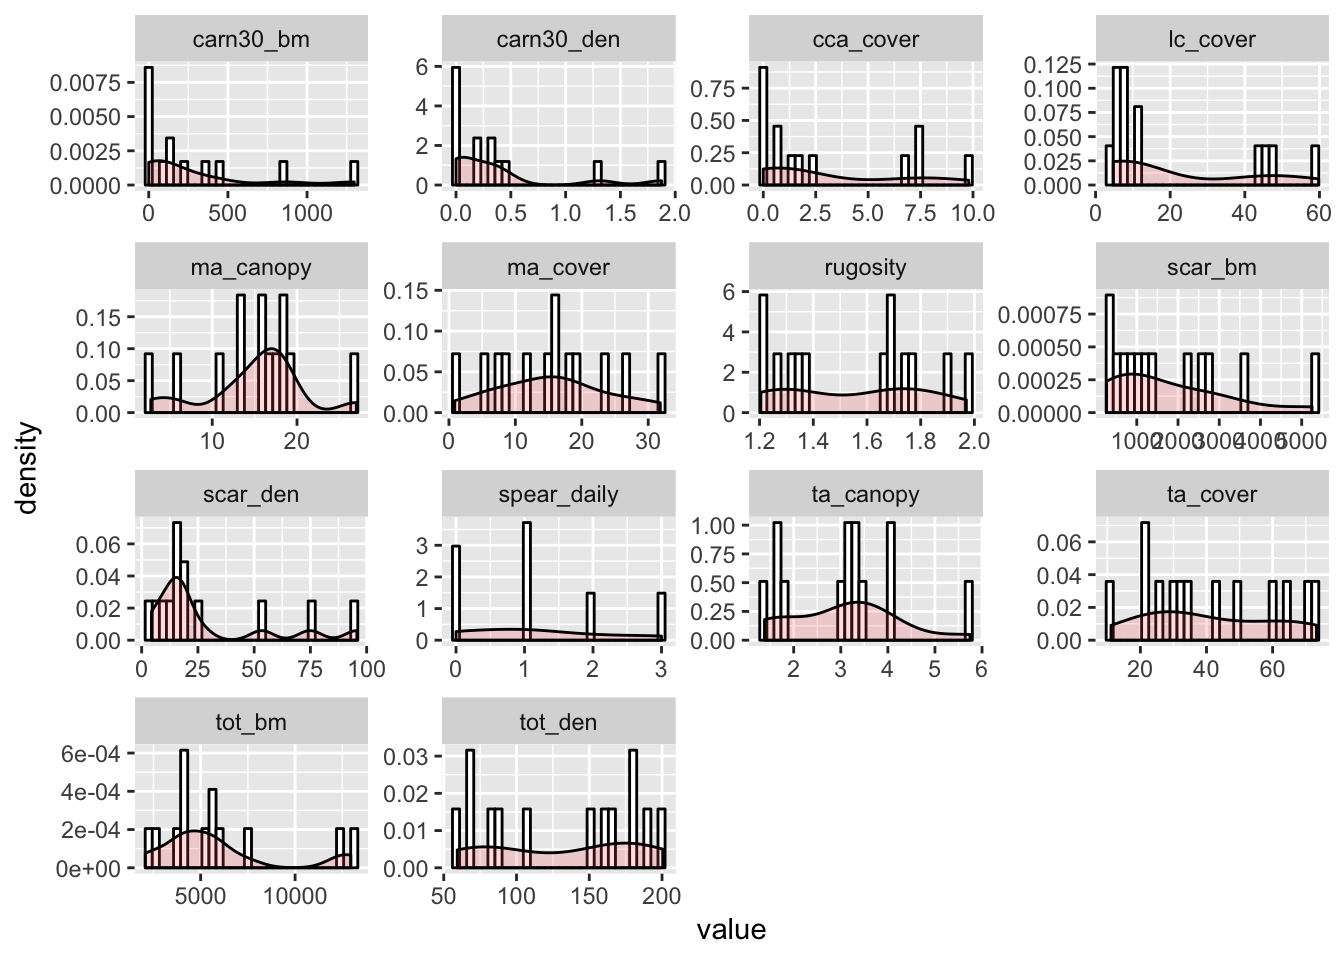
\includegraphics{Ch2_outline_V2_files/figure-latex/unnamed-chunk-2-1.pdf}

\subsection{Variation in feeding rate across benthic and fish community
variables}\label{variation-in-feeding-rate-across-benthic-and-fish-community-variables}

\begin{itemize}
\tightlist
\item
  Initial phase only
\item
  Don't need to include all of these
\item
  Total scarid density, conspecific density, and predator biomass had
  even more variance - didn't include here for scaling purposes but
  ultimately might want to add back in even variables with no
  discernable trend?
\end{itemize}

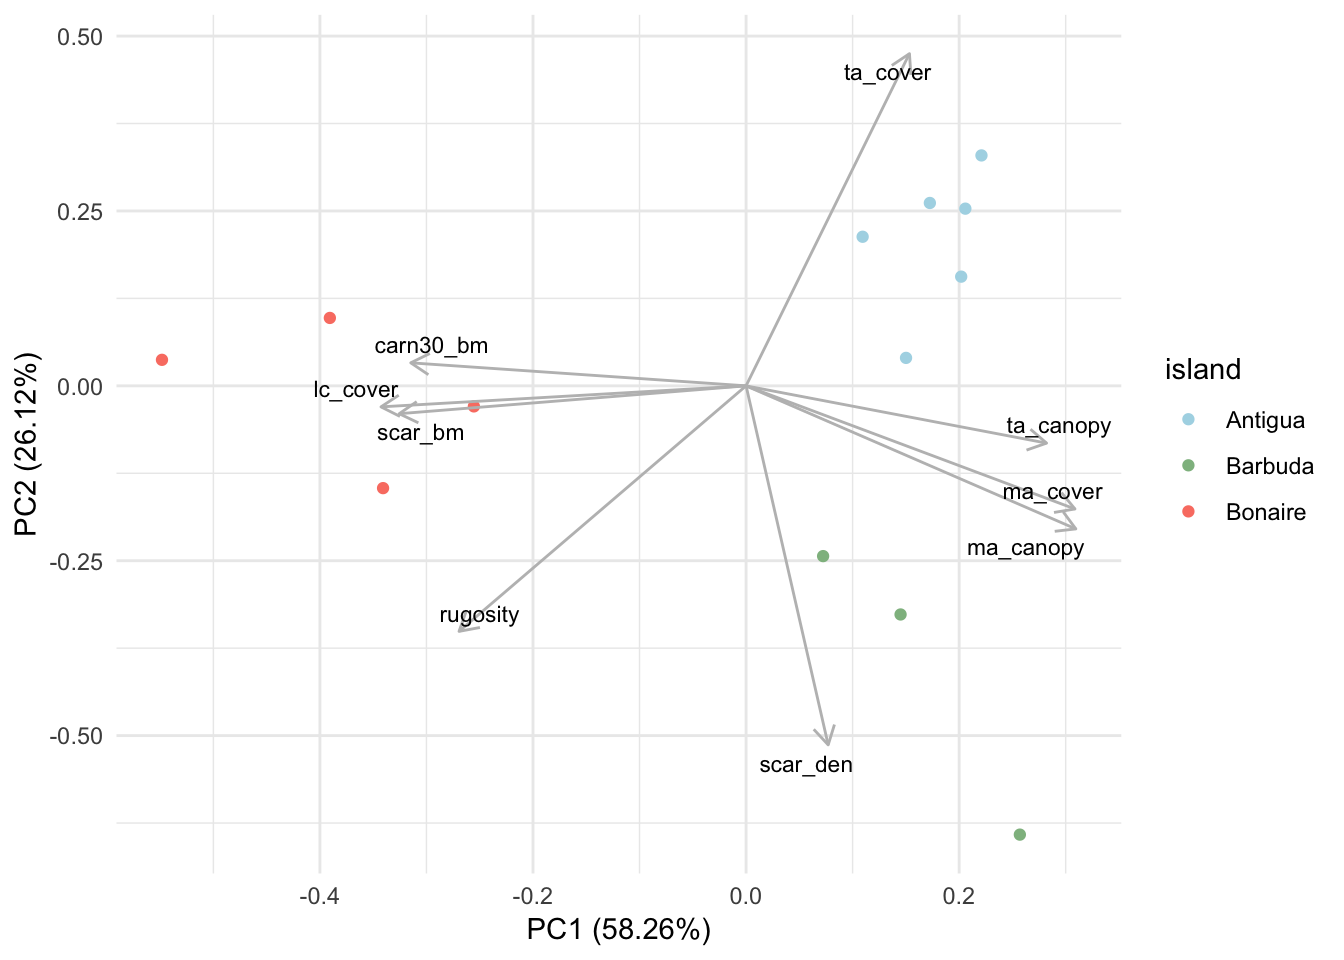
\includegraphics{Ch2_outline_V2_files/figure-latex/unnamed-chunk-3-1.pdf}

\subsection{Variation in feeding intensity across benthic and fish
community
variables}\label{variation-in-feeding-intensity-across-benthic-and-fish-community-variables}

\emph{\emph{Note:} Probably not useful to show both feeding rate and
feeding intensity graphs as trends are very similar\ldots{} but does
have potential impacts on grazing concentration which has potential
ecological relevance. But maybe can show that this varies across sites
without showing all the driver biplots}
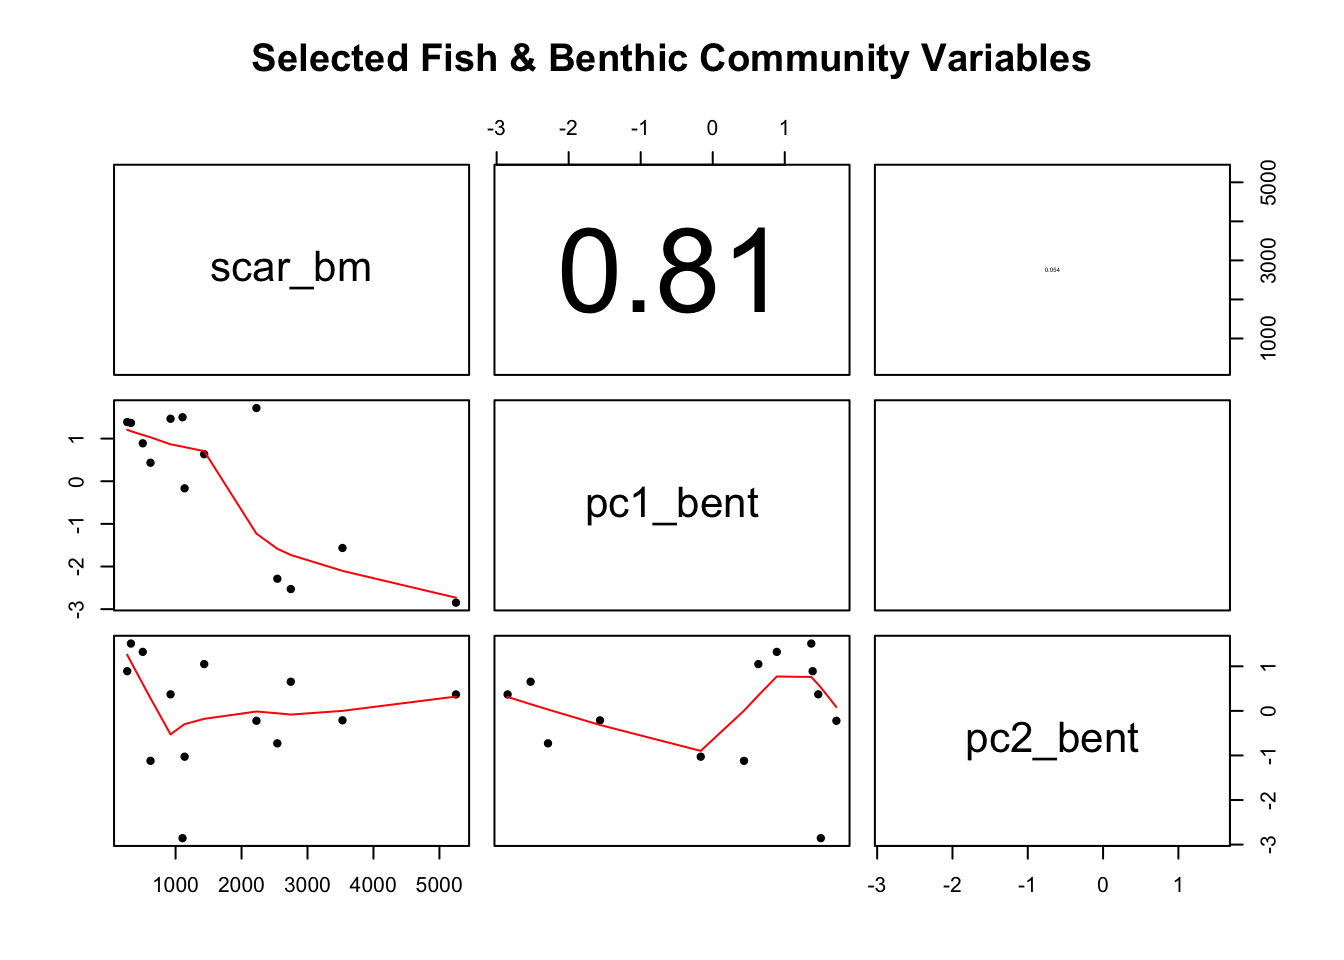
\includegraphics{Ch2_outline_V2_files/figure-latex/unnamed-chunk-4-1.pdf}

\subsection{PCA}\label{pca}

\includegraphics{Ch2_outline_V2_files/figure-latex/unnamed-chunk-5-1.pdf}
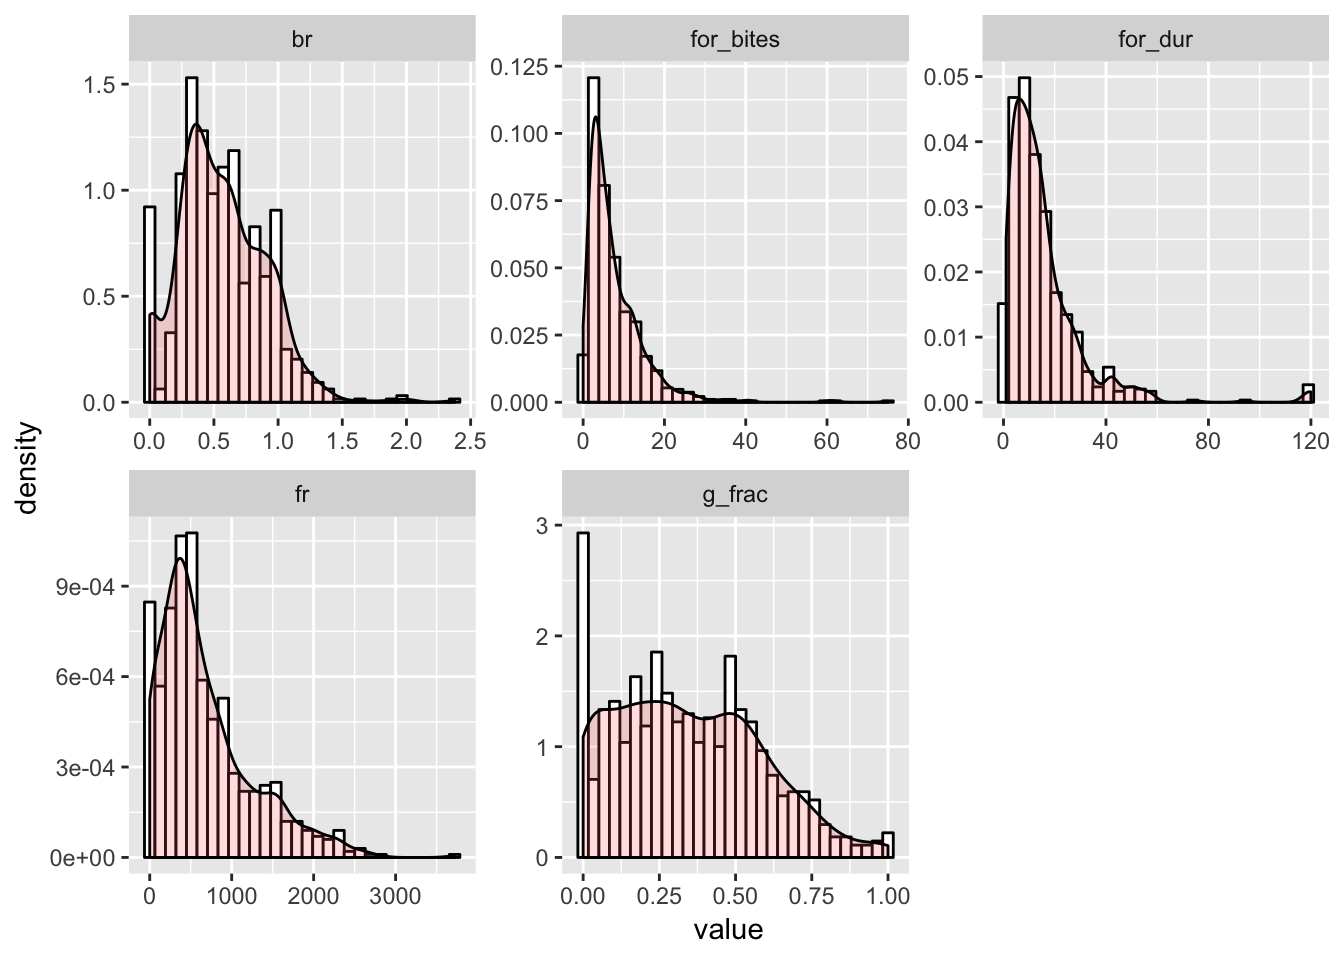
\includegraphics{Ch2_outline_V2_files/figure-latex/unnamed-chunk-6-1.pdf}

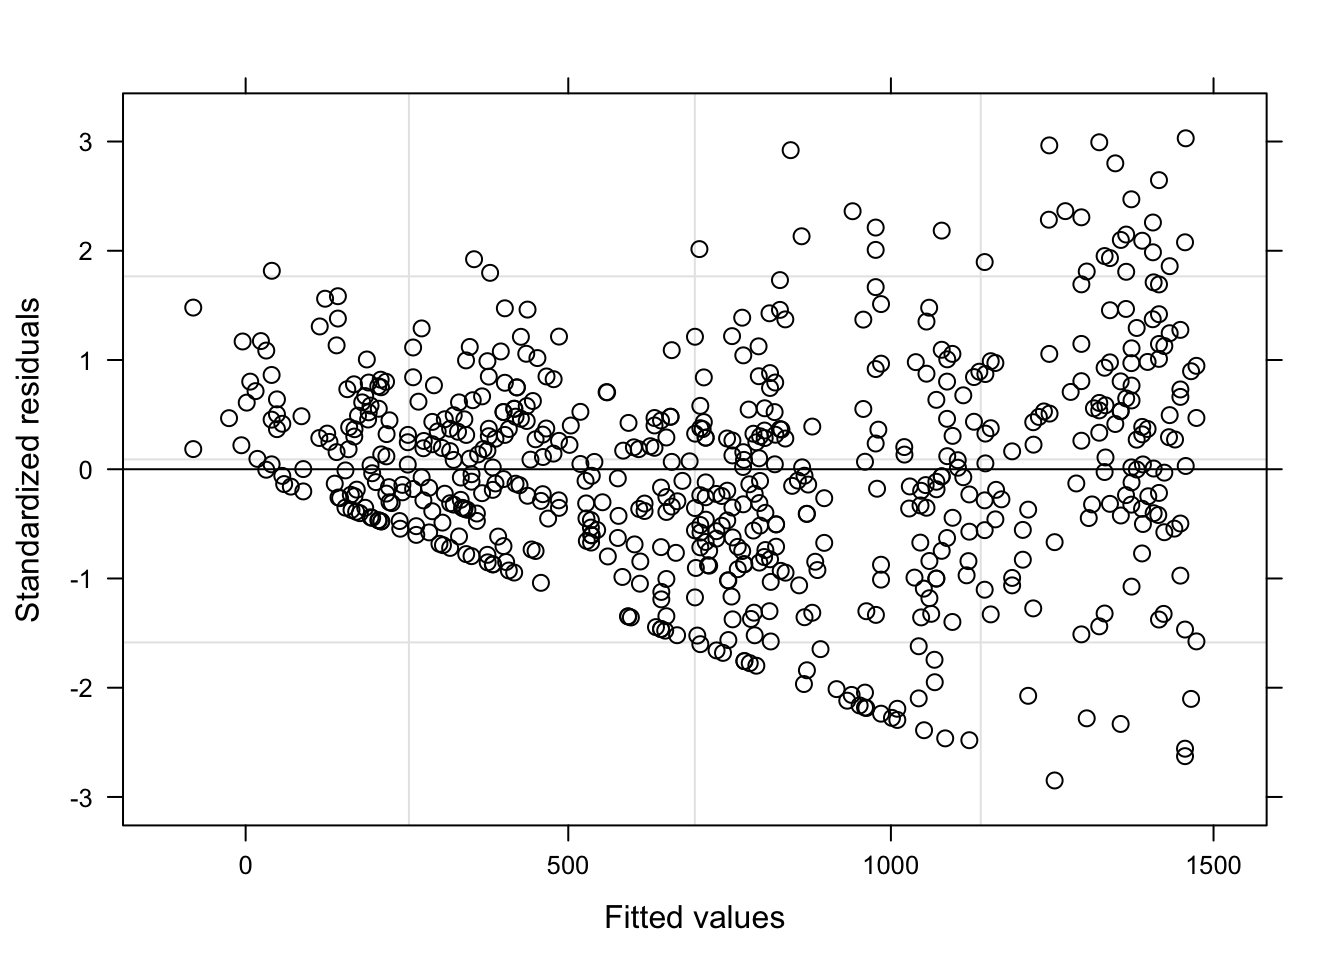
\includegraphics{Ch2_outline_V2_files/figure-latex/unnamed-chunk-7-1.pdf}

\subsection{GAMM results}\label{gamm-results}

One of the GAMM iterations - has lowest AICc, eventually would present
table with other trials/results.

\begin{verbatim}
## 
## Family: gaussian 
## Link function: identity 
## 
## Formula:
## fr_mean ~ species_code + phase + s(length_m, by = factor(species_code), 
##     k = -1) + s(pc1_all, by = factor(species_code), k = -1) + 
##     s(pc2_all, k = -1)
## 
## Parametric coefficients:
##                  Estimate Std. Error t value Pr(>|t|)    
## (Intercept)        979.81     111.33   8.801 1.88e-10 ***
## species_codestop  -403.63      62.63  -6.444 1.89e-07 ***
## phaset            -309.86     115.19  -2.690   0.0108 *  
## ---
## Signif. codes:  0 '***' 0.001 '**' 0.01 '*' 0.05 '.' 0.1 ' ' 1
## 
## Approximate significance of smooth terms:
##                                        edf Ref.df     F  p-value    
## s(length_m):factor(species_code)qup  3.755  3.755 2.392 0.041677 *  
## s(length_m):factor(species_code)stop 1.000  1.000 2.678 0.110417    
## s(pc1_all):factor(species_code)qup   2.719  2.718 7.031 0.000919 ***
## s(pc1_all):factor(species_code)stop  1.000  1.000 0.000 0.995405    
## s(pc2_all)                           1.000  1.000 0.018 0.894012    
## ---
## Signif. codes:  0 '***' 0.001 '**' 0.01 '*' 0.05 '.' 0.1 ' ' 1
## 
## R-sq.(adj) =  0.723   
##   Scale est. = 39781     n = 48
\end{verbatim}

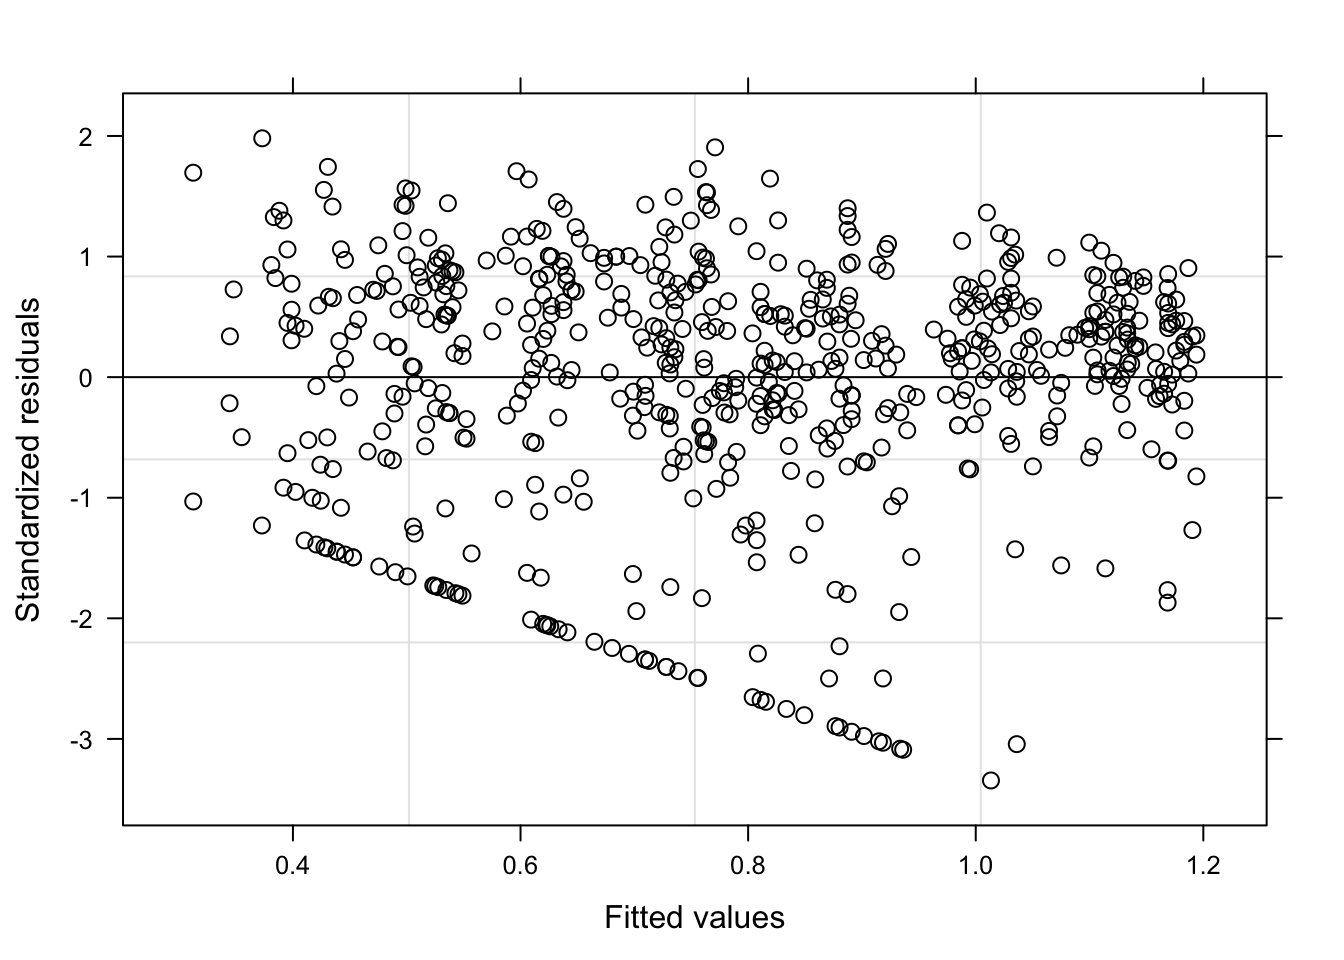
\includegraphics{Ch2_outline_V2_files/figure-latex/unnamed-chunk-9-1.pdf}

\begin{verbatim}
## 
## Family: gaussian 
## Link function: identity 
## 
## Formula:
## fr_mean ~ species_code + phase + s(length_m, by = factor(species_code), 
##     k = 3) + s(pc1_all, by = factor(species_code), k = 3) + s(pc2_all, 
##     k = 3)
## 
## Parametric coefficients:
##                  Estimate Std. Error t value Pr(>|t|)    
## (Intercept)       1001.42     139.66   7.170 1.38e-08 ***
## species_codestop  -387.76      67.45  -5.749 1.22e-06 ***
## phaset            -365.91     119.27  -3.068  0.00394 ** 
## ---
## Signif. codes:  0 '***' 0.001 '**' 0.01 '*' 0.05 '.' 0.1 ' ' 1
## 
## Approximate significance of smooth terms:
##                                        edf Ref.df     F p-value  
## s(length_m):factor(species_code)qup  1.886  1.886 3.551  0.0301 *
## s(length_m):factor(species_code)stop 1.000  1.000 3.369  0.0741 .
## s(pc1_all):factor(species_code)qup   1.772  1.772 7.410  0.0141 *
## s(pc1_all):factor(species_code)stop  1.000  1.000 0.566  0.4566  
## s(pc2_all)                           1.000  1.000 0.354  0.5553  
## ---
## Signif. codes:  0 '***' 0.001 '**' 0.01 '*' 0.05 '.' 0.1 ' ' 1
## 
## R-sq.(adj) =  0.591   
##   Scale est. = 47706     n = 48
\end{verbatim}

\includegraphics{Ch2_outline_V2_files/figure-latex/unnamed-chunk-9-2.pdf}

\subsection{Bite content hypothesis}\label{bite-content-hypothesis}

\begin{Shaded}
\begin{Highlighting}[]
\CommentTok{# grazing impact of fish from behavioral surveys}
\NormalTok{sum_id_vg <-}\StringTok{ }\NormalTok{sum_id }\OperatorTok
\StringTok{  }\KeywordTok{filter}\NormalTok{(species_code }\OperatorTok{!=}\StringTok{ "rbp"}\NormalTok{) }\OperatorTok
\StringTok{  }\KeywordTok{mutate}\NormalTok{(}
    \DataTypeTok{bs =} \KeywordTok{ifelse}\NormalTok{(species_code }\OperatorTok{==}\StringTok{ "stop"}\NormalTok{, }\FloatTok{5.257}\OperatorTok{*}\DecValTok{10}\OperatorTok{^-}\DecValTok{4}\OperatorTok{*}\NormalTok{length_cm}\OperatorTok{^}\DecValTok{2}\NormalTok{, }\FloatTok{4.013}\OperatorTok{*}\DecValTok{10}\OperatorTok{^-}\DecValTok{4}\OperatorTok{*}\NormalTok{length_cm}\OperatorTok{^}\DecValTok{2}\NormalTok{), }\CommentTok{# adding bite size equations from Mumby}
    \DataTypeTok{bh_capped =} \KeywordTok{ifelse}\NormalTok{(ta_canopy }\OperatorTok{<}\StringTok{ }\DecValTok{2}\OperatorTok{*}\KeywordTok{sqrt}\NormalTok{(bs)}\OperatorTok{/}\NormalTok{(}\DecValTok{22}\OperatorTok{/}\DecValTok{7}\NormalTok{), ta_canopy, }\DecValTok{2}\OperatorTok{*}\KeywordTok{sqrt}\NormalTok{(bs)}\OperatorTok{/}\NormalTok{(}\DecValTok{22}\OperatorTok{/}\DecValTok{7}\NormalTok{)), }\CommentTok{# if ta_canopy exceeds diameter of bite size, bite height is capped at bite size}
    \DataTypeTok{bv =}\NormalTok{ bs}\OperatorTok{*}\NormalTok{ta_canopy,}
    \DataTypeTok{bv_capped =}\NormalTok{ bs}\OperatorTok{*}\NormalTok{bh_capped,}
    \DataTypeTok{vg =}\NormalTok{ fr}\OperatorTok{*}\NormalTok{bv,}
    \DataTypeTok{vg_capped =}\NormalTok{ fr}\OperatorTok{*}\NormalTok{bv_capped,}
    \DataTypeTok{island =} \KeywordTok{factor}\NormalTok{(island, }\DataTypeTok{levels =} \KeywordTok{c}\NormalTok{(}\StringTok{"Bonaire"}\NormalTok{,}\StringTok{"Antigua"}\NormalTok{,}\StringTok{"Barbuda"}\NormalTok{))}
\NormalTok{) }\OperatorTok
\StringTok{  }\KeywordTok{arrange}\NormalTok{(island)}

\NormalTok{sum_ssp_vg <-}\StringTok{ }\NormalTok{sum_id_vg }\OperatorTok\StringTok{ }
\StringTok{  }\KeywordTok{group_by}\NormalTok{(site, island, species, species_code, phase) }\OperatorTok\StringTok{ }
\StringTok{  }\KeywordTok{summarize}\NormalTok{(}
    \DataTypeTok{n=}\KeywordTok{n}\NormalTok{(),}
    \DataTypeTok{vg_mean=}\KeywordTok{mean}\NormalTok{(vg),}
    \DataTypeTok{vg_se=}\KeywordTok{sd}\NormalTok{(vg)}\OperatorTok{/}\KeywordTok{sqrt}\NormalTok{(n),}
    \DataTypeTok{vg_capped_mean=}\KeywordTok{mean}\NormalTok{(vg_capped),}
    \DataTypeTok{vg_capped_se=}\KeywordTok{sd}\NormalTok{(vg_capped)}\OperatorTok{/}\KeywordTok{sqrt}\NormalTok{(n)}
\NormalTok{    ) }\OperatorTok\StringTok{ }
\StringTok{  }\KeywordTok{select}\NormalTok{(}\OperatorTok{-}\NormalTok{n)}

\KeywordTok{ggplot}\NormalTok{(}\KeywordTok{filter}\NormalTok{(sum_ssp_vg, species_code }\OperatorTok{!=}\StringTok{ "rbp"} \OperatorTok{&}\StringTok{ }\NormalTok{phase }\OperatorTok{==}\StringTok{ "i"}\NormalTok{), }\KeywordTok{aes}\NormalTok{(}\DataTypeTok{x=}\KeywordTok{factor}\NormalTok{(site, }\DataTypeTok{levels =}\NormalTok{ sum_site}\OperatorTok{$}\NormalTok{site), }\DataTypeTok{y=}\NormalTok{vg_mean)) }\OperatorTok{+}
\StringTok{    }\KeywordTok{geom_bar}\NormalTok{(}\DataTypeTok{stat =} \StringTok{"identity"}\NormalTok{, }\KeywordTok{aes}\NormalTok{(}\DataTypeTok{fill =}\NormalTok{ island), }\DataTypeTok{position =} \StringTok{"dodge"}\NormalTok{) }\OperatorTok{+}
\StringTok{    }\KeywordTok{geom_errorbar}\NormalTok{(}\KeywordTok{aes}\NormalTok{(}\DataTypeTok{ymin=}\NormalTok{vg_mean}\OperatorTok{-}\NormalTok{vg_se, }\DataTypeTok{ymax=}\NormalTok{vg_mean}\OperatorTok{+}\NormalTok{vg_se), }\DataTypeTok{width=}\NormalTok{.}\DecValTok{2}\NormalTok{,}
                 \DataTypeTok{position=}\KeywordTok{position_dodge}\NormalTok{(.}\DecValTok{9}\NormalTok{)) }\OperatorTok{+}
\StringTok{    }\KeywordTok{facet_grid}\NormalTok{(}\OperatorTok{~}\NormalTok{species) }\OperatorTok{+}
\StringTok{    }\KeywordTok{scale_fill_brewer}\NormalTok{(}\DataTypeTok{palette =} \StringTok{"Blues"}\NormalTok{) }\OperatorTok{+}
\StringTok{    }\KeywordTok{labs}\NormalTok{(}\DataTypeTok{title=}\StringTok{"Mean grazing impact by volume (initial phase)"}\NormalTok{, }
         \DataTypeTok{y=}\StringTok{"Grazing impact (cm3/hr)"}\NormalTok{, }
         \DataTypeTok{x=}\StringTok{"Site"}\NormalTok{) }\OperatorTok{+}
\StringTok{    }\KeywordTok{theme_bw}\NormalTok{() }\OperatorTok{+}
\StringTok{    }\KeywordTok{theme}\NormalTok{(}\DataTypeTok{strip.text =} \KeywordTok{element_text}\NormalTok{(}\DataTypeTok{face =} \StringTok{"italic"}\NormalTok{), }
          \DataTypeTok{axis.text.x =} \KeywordTok{element_text}\NormalTok{(}\DataTypeTok{angle =} \DecValTok{90}\NormalTok{, }\DataTypeTok{hjust =} \DecValTok{1}\NormalTok{), }
          \DataTypeTok{plot.title =} \KeywordTok{element_text}\NormalTok{(}\DataTypeTok{hjust =} \FloatTok{0.5}\NormalTok{))}
\end{Highlighting}
\end{Shaded}

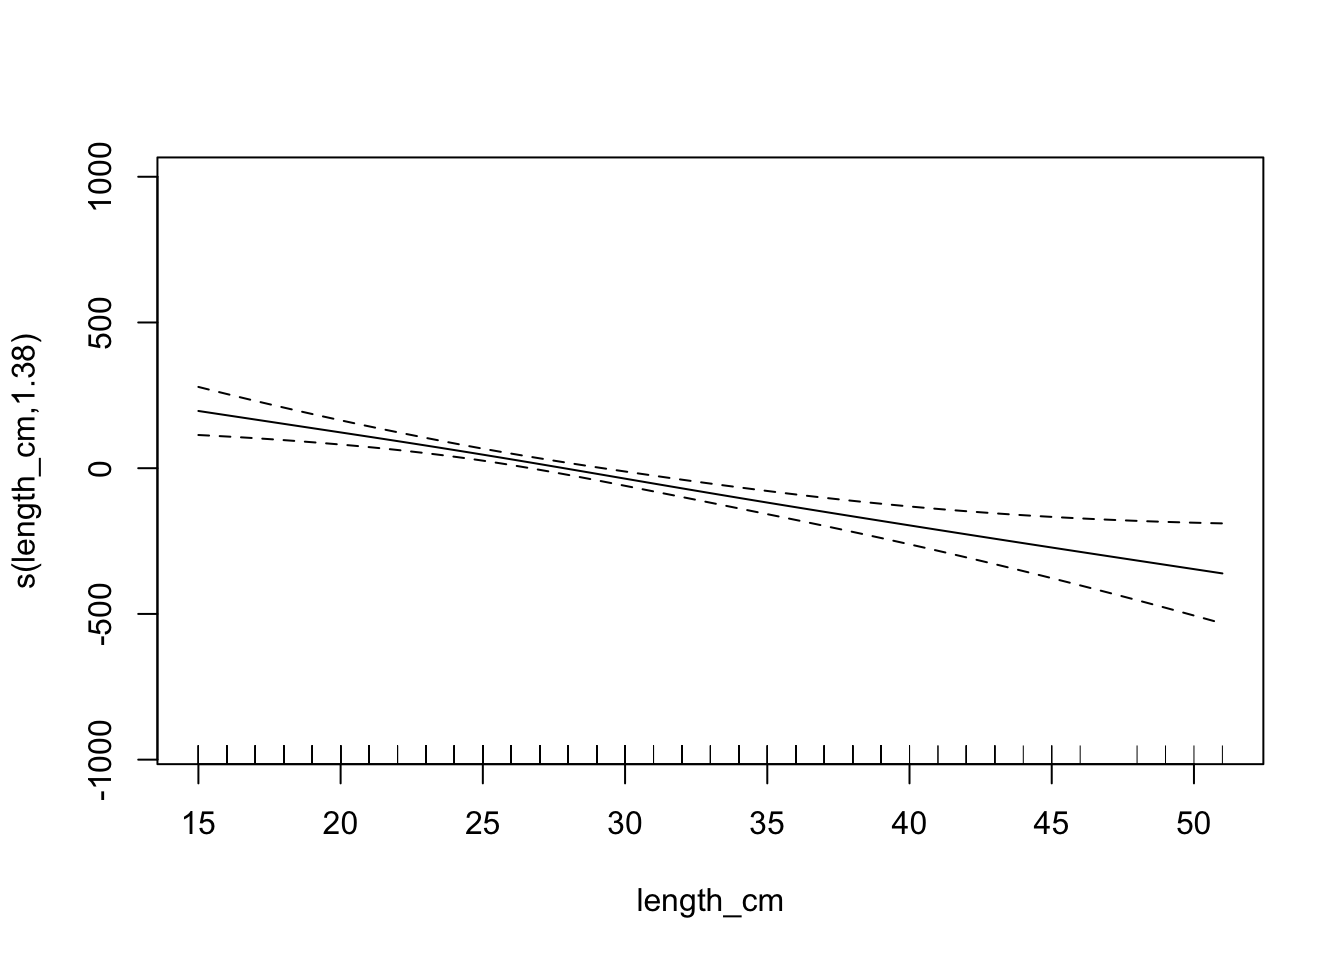
\includegraphics{Ch2_outline_V2_files/figure-latex/unnamed-chunk-10-1.pdf}

\begin{Shaded}
\begin{Highlighting}[]
\KeywordTok{ggplot}\NormalTok{(}\KeywordTok{filter}\NormalTok{(sum_ssp_vg, species_code }\OperatorTok{!=}\StringTok{ "rbp"} \OperatorTok{&}\StringTok{ }\NormalTok{phase }\OperatorTok{==}\StringTok{ "i"}\NormalTok{), }\KeywordTok{aes}\NormalTok{(}\DataTypeTok{x=}\KeywordTok{factor}\NormalTok{(site, }\DataTypeTok{levels =}\NormalTok{ sum_site}\OperatorTok{$}\NormalTok{site), }\DataTypeTok{y=}\NormalTok{vg_capped_mean)) }\OperatorTok{+}
\StringTok{    }\KeywordTok{geom_bar}\NormalTok{(}\DataTypeTok{stat =} \StringTok{"identity"}\NormalTok{, }\KeywordTok{aes}\NormalTok{(}\DataTypeTok{fill =}\NormalTok{ island), }\DataTypeTok{position =} \StringTok{"dodge"}\NormalTok{) }\OperatorTok{+}
\StringTok{    }\KeywordTok{geom_errorbar}\NormalTok{(}\KeywordTok{aes}\NormalTok{(}\DataTypeTok{ymin=}\NormalTok{vg_capped_mean}\OperatorTok{-}\NormalTok{vg_capped_se, }\DataTypeTok{ymax=}\NormalTok{vg_capped_mean}\OperatorTok{+}\NormalTok{vg_capped_se), }\DataTypeTok{width=}\NormalTok{.}\DecValTok{2}\NormalTok{,}
                 \DataTypeTok{position=}\KeywordTok{position_dodge}\NormalTok{(.}\DecValTok{9}\NormalTok{)) }\OperatorTok{+}
\StringTok{    }\KeywordTok{facet_grid}\NormalTok{(}\OperatorTok{~}\NormalTok{species) }\OperatorTok{+}
\StringTok{    }\KeywordTok{scale_fill_brewer}\NormalTok{(}\DataTypeTok{palette =} \StringTok{"Blues"}\NormalTok{) }\OperatorTok{+}
\StringTok{    }\KeywordTok{labs}\NormalTok{(}\DataTypeTok{title=}\StringTok{"Mean grazing impact by volume (capped height, initial phase)"}\NormalTok{, }
         \DataTypeTok{y=}\StringTok{"Grazing impact (cm3/hr)"}\NormalTok{, }
         \DataTypeTok{x=}\StringTok{"Site"}\NormalTok{) }\OperatorTok{+}
\StringTok{    }\KeywordTok{theme_bw}\NormalTok{() }\OperatorTok{+}
\StringTok{    }\KeywordTok{theme}\NormalTok{(}\DataTypeTok{strip.text =} \KeywordTok{element_text}\NormalTok{(}\DataTypeTok{face =} \StringTok{"italic"}\NormalTok{), }
          \DataTypeTok{axis.text.x =} \KeywordTok{element_text}\NormalTok{(}\DataTypeTok{angle =} \DecValTok{90}\NormalTok{, }\DataTypeTok{hjust =} \DecValTok{1}\NormalTok{), }
          \DataTypeTok{plot.title =} \KeywordTok{element_text}\NormalTok{(}\DataTypeTok{hjust =} \FloatTok{0.5}\NormalTok{))}
\end{Highlighting}
\end{Shaded}

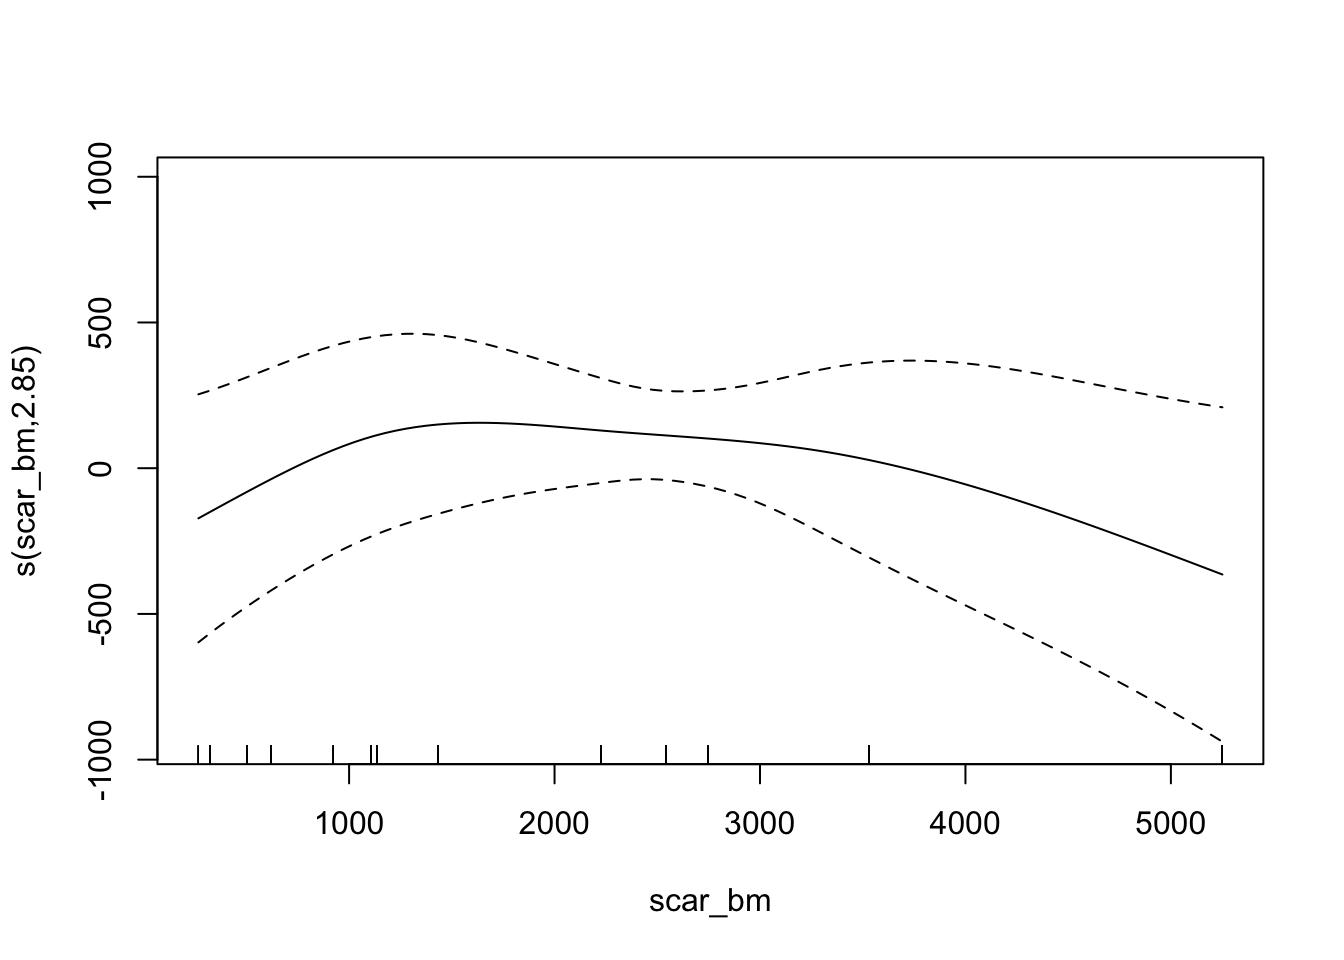
\includegraphics{Ch2_outline_V2_files/figure-latex/unnamed-chunk-10-2.pdf}

\section{Discussion}\label{discussion}

\begin{itemize}
\tightlist
\item
  Significant differences in feeding behaviors within species across
  islands (be conservative about conclusions here, just presenting
  observed trends despite relatively small sample sizes)
\item
  GAMM results: explain meaning/significance of PC1 (essentially higher
  feeding rates in reefs with higher scarid biomass and rugosity
  vs.~more algal dominated and lower scarid biomass reefs); \emph{S.
  vetula} seem more impacted by PC1 than \emph{S. viride}.
\item
  Potential mechanisms/hypotheses for these observed trends:

  \begin{itemize}
  \tightlist
  \item
    Social feeding hypothesis: more time must be spent vigilant in
    smaller groups, potential compounding effect with overfishing/loss
    of herbivory
  \item
    Nutrient limitation hypothesis: scarids must graze more (and more
    intensely) in sites with lower algal canopy heights and percent
    cover
  \item
    Predation risk hypothesis: presence of large piscivores does not
    explain feeding trends, but risk from spearfishers may play a bigger
    role (able to target larger fish, i.e.~those sampled here).
    (Incorporate rugosity here - Rogers, Madin, Catano)
  \end{itemize}
\item
  Ecological implications: potential reinforcing feedback loops in
  degraded reefs if high algal/low scarid reefs also have less grazing
  impact per scarid

  \begin{itemize}
  \tightlist
  \item
    Feeding intensity: less intense feeding/more distributed bites in
    degraded reefs may also reduce actual substrate made available to
    recruiting corals (\textasciitilde{} grazing concentration lit.
    here)
  \end{itemize}
\item
  Caveats + limitations: all these potential drivers/mechanisms are
  understandably correlated in observational work

  \begin{itemize}
  \tightlist
  \item
    Room for experimental work to unpack/distinguish drivers
  \end{itemize}
\item
  Need for incorporation of behavior in coral reef grazing models,
  especially those used to set targets for minimum herbivore biomass
  levels, because these may look very different in different reef
  conditions. Current paradigm of constant species-level grazing
  behaviors may be inaccurate. In Caribbean case, most models use
  Bonaire data which may not be representative of dynamics on more
  degraded Caribbean reefs.
\item
  Need for framework to help incorporate behavioral effects into
  ecosystem management
\item
  Conservation + mgmt implications: multiple human impacts on reefs may
  affect herbivore behavior in different ways, spec. fishing + habitat
  degradation - which may have reinforcing/compounding negative effects
  on reef health
\end{itemize}


\end{document}
